\section{Runtime View}
\subsection{Runtime Overview}

\begin{figure}[ht]
  \centering
  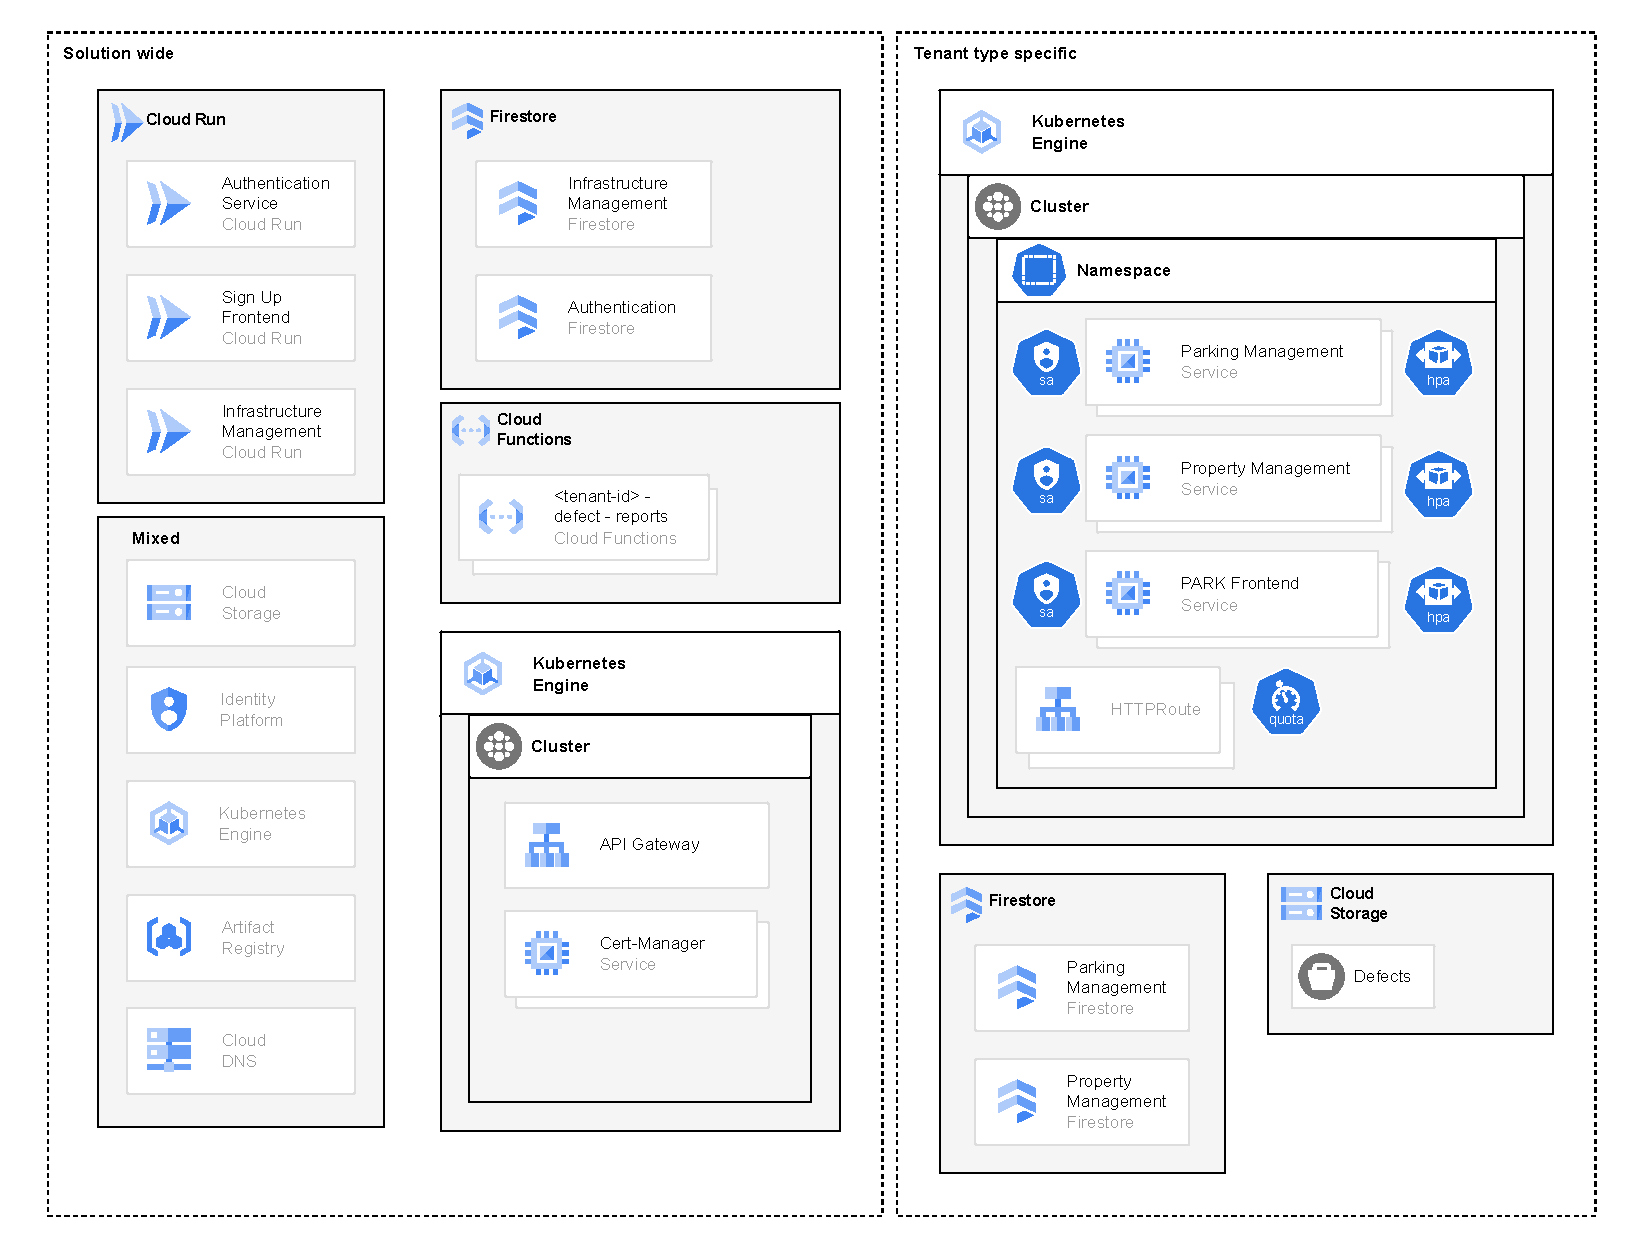
\includegraphics[width=\textwidth]{resources/03-runtime-view/pdf/cloud-ressources.pdf}
  \caption{Übersicht über die Cloud Ressourcen}
  \label{fig:cloud-ressources}
\end{figure}

\begin{figure}[ht]
  \centering
  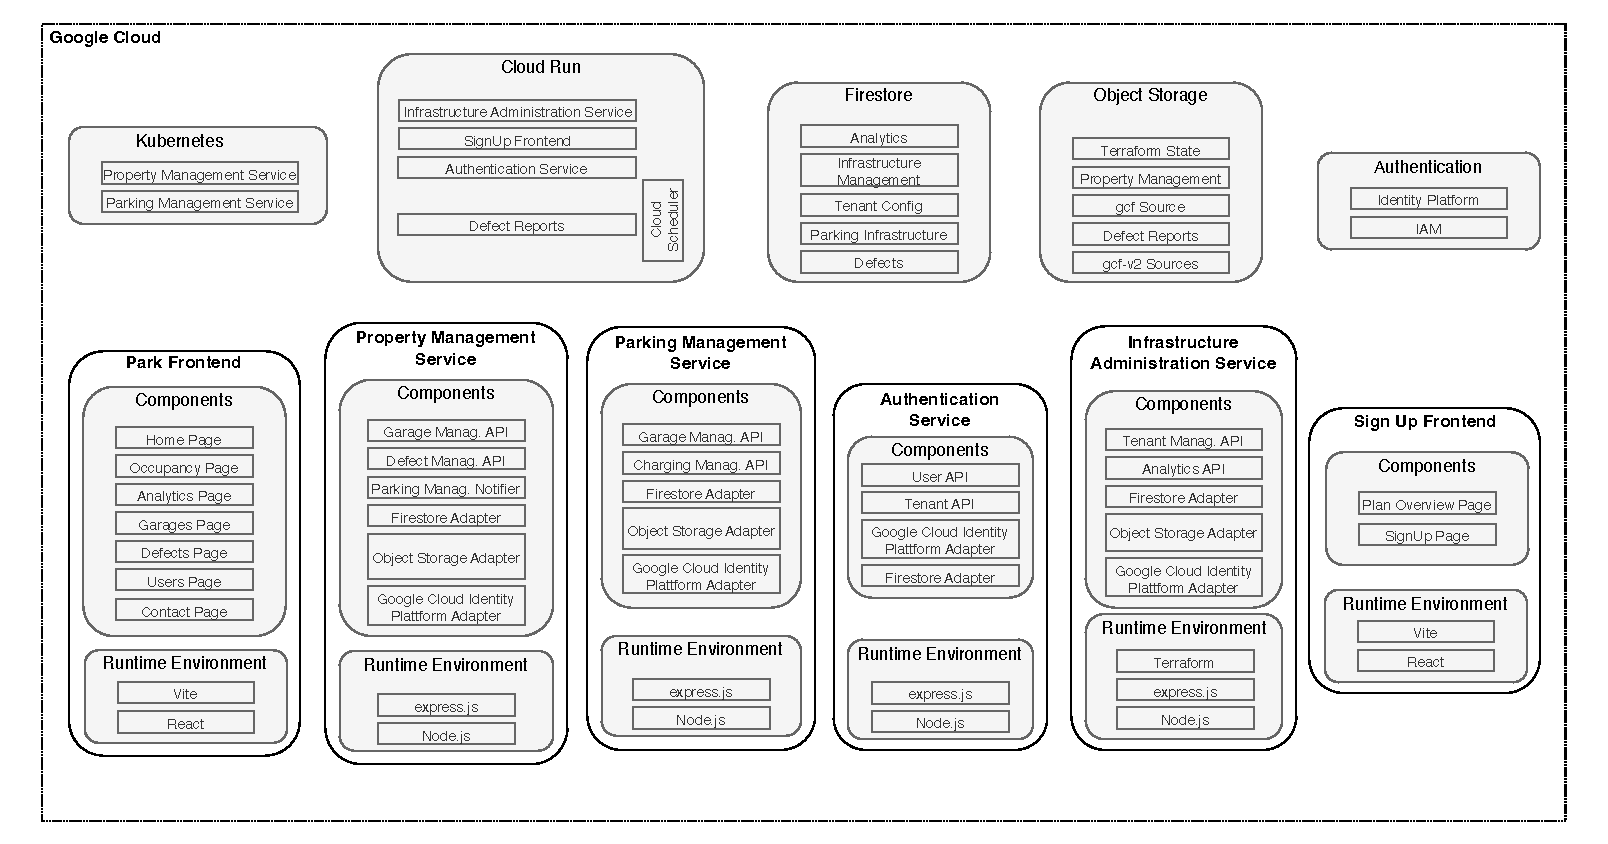
\includegraphics[width=\textwidth]{resources/03-runtime-view/pdf/architecture.pdf}
  \caption{Alle Mircoservices}
  \label{fig:system-architecture}
\end{figure}

In Abbildung~\ref{fig:cloud-ressources} werden alle verwendeten Cloud Ressourcen unterteilt in zwei Gruppen dargestellt:
\paragraph{Anwendungweite Ressources} sind Ressourcen, die von allen Tenants gemeinsam genutzt werden. 
Diese Ressourcen unterteilen sich nochmal in folgende Kategorien:
\begin{itemize}
  \item \textbf{Cloud Run} - Alle Services, welche in Cloud Run laufen. (Authentication Service, Infrastructure Management Service \& Sign Up Frontend)
  \item \textbf{Firestore} - Die Firestore Datenbanken, welche von den Cloud Run Services benötigt werden.
  \item \textbf{Cloud Functions} - Pro Tenant gibt es eine Defect-Report Cloud Function.
  \item \textbf{Mixed} - Weitere Cloud Ressourcen, welche für den Betrieb unsere Anwendung benötigt werden. (z.B. Cloud Storage, Identity Platform, Kubernetes Engine, Artifact Registry \& Ingres / DNS) 
\end{itemize}

\paragraph{Tenant Typ spezifische Ressources} sind Ressourcen, die sich von allen Tenants des selben Tenant Typs geteilt werden.
Jeder Enterprise Tenant wird hierbei als eigener Tenant Typ betrachtet, um die verwendeten Ressourcen bessere darstellen und erklären zu können. 
Die Ressourcen unterteilen sich nochmal in folgende Kategorien:
\begin{itemize}
  \item \textbf{Kubernetes} - Innerhalb der annwedungsweiten Kubernetes Engine existiert ein Cluster. Innerhalb des Cluster wird pro Tenant Typ ein neuer Namespace angelegt, in welchem die Services (Property Management \& Parking Management) laufen, welche sich alle Tenants eines Typs teilen.
  \item \textbf{Firestore} - Die Firestore Datenbanken, welche für die Services im Tenant Typ spezifischen Namespace benötigt werden. (Property Management \& Parking Management)
  \item \textbf{Cloud Storage} - Für den Property Management Service wird ein eigener Bucket angelegt, um die Bilder der Defects speichern zu können.
\end{itemize}

Um die Interaktionen zwischen den Komponenten als auch den anwendungweiten und Tenant Typ spezifischen Ressourcen zu verdeutlichen, wird in Abbildung~\ref{fig:system-architecture} die gesamte Systemarchitektur dargestellt. Hier sieht man, wie sich alle Komponenten eine Authentication Service und Infrastructure Management Service Instanz teilen.

\begin{figure}[ht]
  \centering
  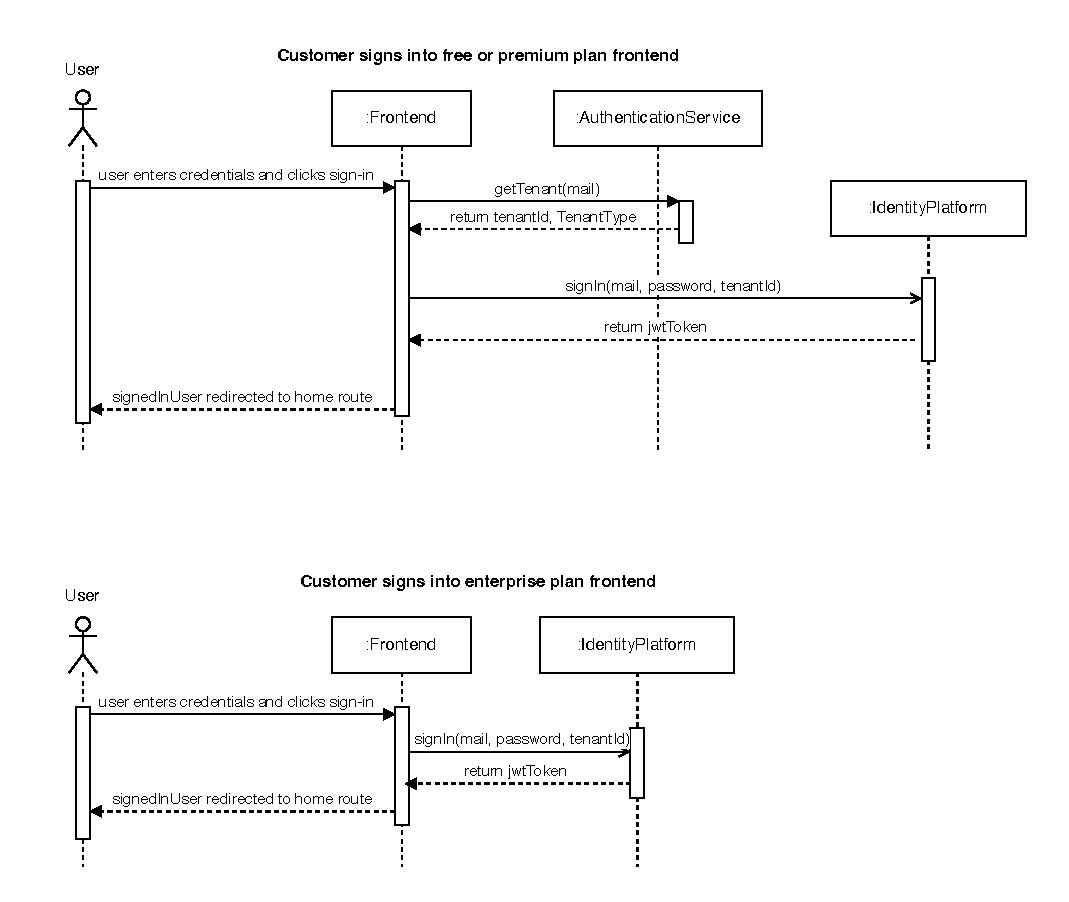
\includegraphics[width=\textwidth]{resources/03-runtime-view/pdf/authentication-sequence.pdf}
  \caption{Ablauf der Tenant Typ abhängigen Authentifizierung}
  \label{fig:authentication-sequence}
\end{figure}

Eine Besonderheit ist hierbei die Authentifizierung mittels Authentication Service und Identity Platform. In Abbildung~\ref{fig:authentication-sequence} wird der Ablauf der Authentifizierung dargestellt. Das heißt wenn sich ein Nutzer in seiner Tenant Typ spezifischen Instanz des Frontends anmeldet, wird zuerst über den Authentication Service abgefragt, ob der Nutzer überhaupt vom richtigen Tenant Typ ist und falls ja die Tenant Id, zu welchem der Nutzer gehört. Anschließend wird der Nutzer Tenant-Aware über die Identity Platform authentifiziert. Wenn die Authentifizierung erfolgreich war, wird der Nutzer auf die entsprechende Home-Seite weitergeleitet und im Hintergrund im Local-Storage ein JWT Token zu Authentifizierung im Backend abgelegt. 
Für den Tenant Typ Enterprise entfällt die Anfrage an den Authentication Service, da diese Frontend nur von einem Tenant verwendet wird und daher die Tenant Id als Konstante im Environment hinterlegt ist.

\begin{figure}[ht]
  \centering
  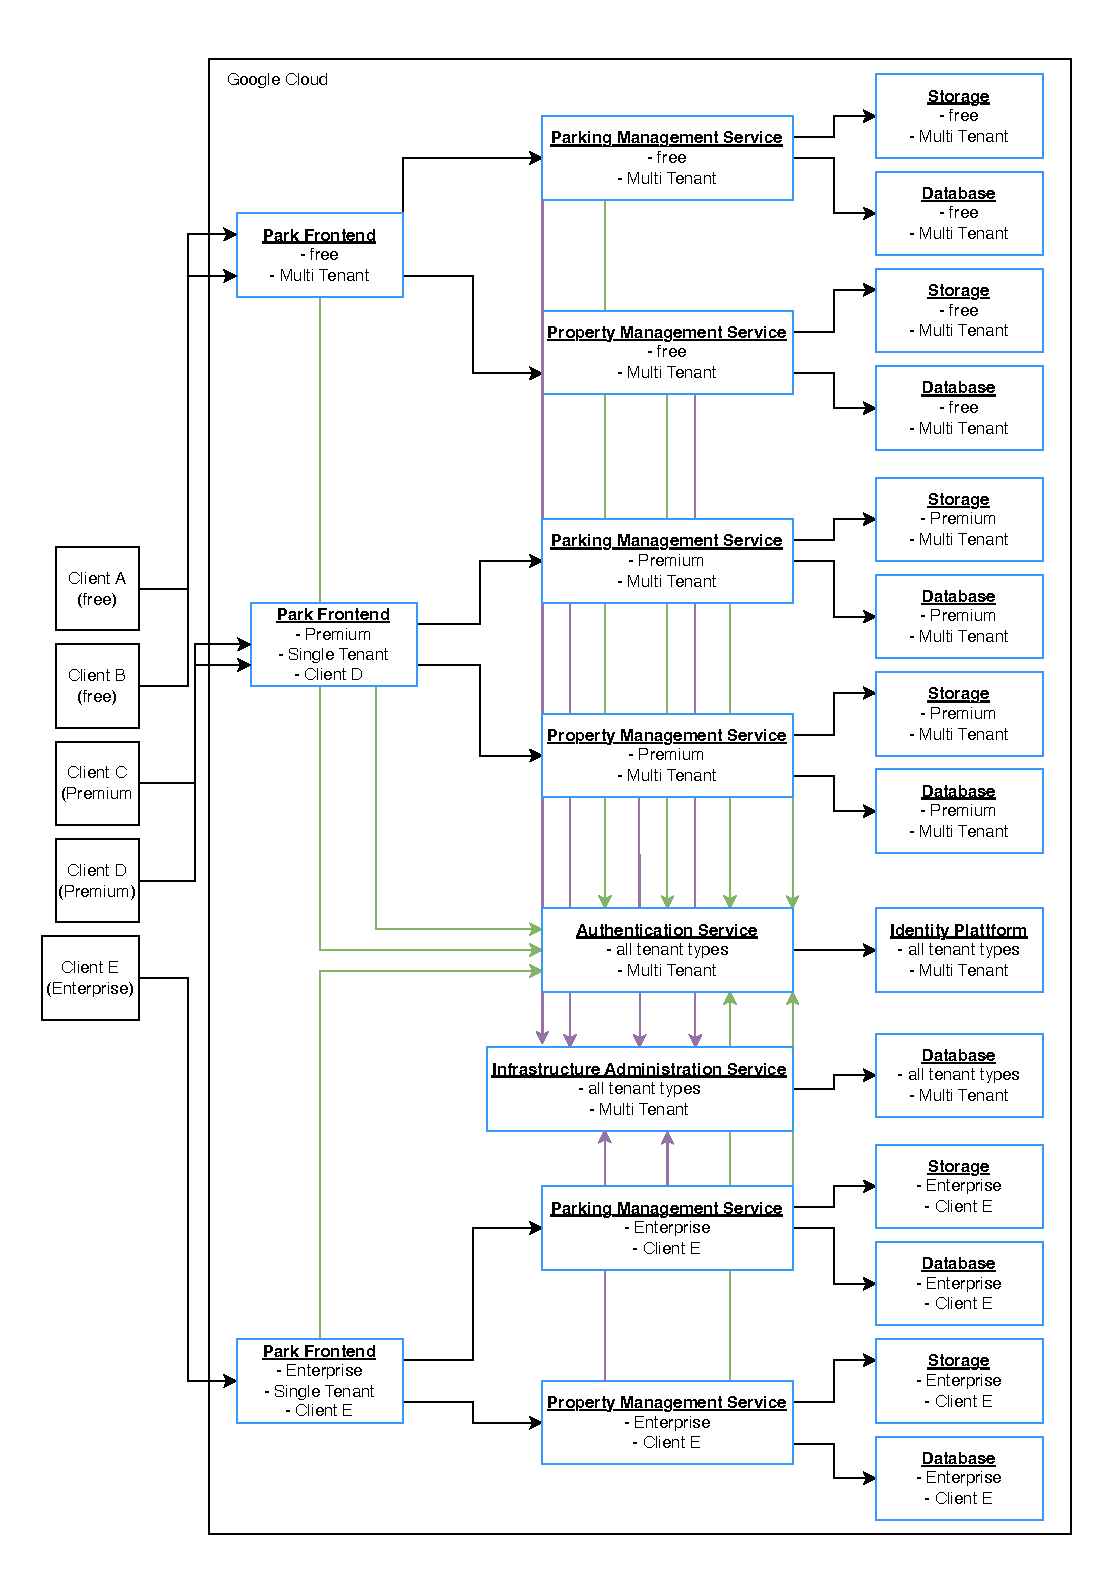
\includegraphics[width=0.95\textwidth]{resources/03-runtime-view/pdf/components-frontend-park.pdf}
  \caption{Alle verwendeten Komponenten, wenn ein Client mit dem Park Frontend interagiert, mit Berücksichtigung von Multitenancy}
  \label{fig:components-park-frontend}
\end{figure}

\begin{figure}[ht]
  \centering
  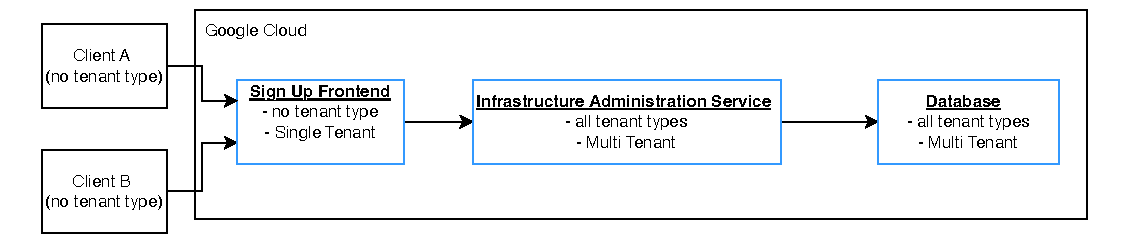
\includegraphics[width=\textwidth]{resources/03-runtime-view/pdf/components-frontend-signup.pdf}
  \caption{Alle verwendeten Komponenten, wenn ein Client mit dem Signup Frontend interagiert}
  \label{fig:components-signup-frontend}
\end{figure}

\subsection{Mircoservices}

In Abbildung~\ref{fig:components-park-frontend} und Abbildung~\ref{fig:components-signup-frontend} werden alle Komponenten dargestellt, welche bei einer Interaktion mit dem Park Frontend oder dem Sign Up Frontend verwendet werden.
% TODO: Runtime Konfiguration
% TODO: Scaling
% TODO: Customization
% TODO: Security Setup
% TODO: Vbd. zu Datenbanken
\subsection{Data Stores}